\begin{frame}
    \frametitle{Деревья линейных расщеплений (LST)}
	Расщепления по линейным формам над полем $\mathbb{F}_2$
    \begin{columns}
        \begin{column}{3cm}
            Вырожденный лист
            \tikzstyle{end} = [circle, minimum size = 0.1cm, draw, inner sep = 0.1pt]
\tikzstyle{leaf} = [circle, minimum size = 0.6cm, draw, inner sep = 0.1pt, blue]
            
\tikzstyle{level 1}=[level distance = 1cm, sibling distance = 1cm]
\tikzstyle{level 2}=[level distance = 1.5cm, sibling distance = 1.5cm]
\tikzstyle{level 3}=[level distance = 1.5cm, sibling distance = 1.8cm]


    
\begin{tikzpicture}[label distance = 8mm]
	\node [end] (z){}
        child {
        	node[end] (b) {}
            child {
    			node {$\vdots$}
		        edge from parent
	    		node[left] {}
			}
		    child {
		        node[end] {}
                child {
                  	node {\alert{no sol.}}
                    edge from parent
                    node[left] {$y = 0$}
                }
                child {
        			node {$\vdots$}
		           	edge from parent
        		    node[right] {$y = 1$}
		        }
	            edge from parent
		        node[right] {$x + y = 1$}
            }
           	edge from parent
            node[left] {$x = 0$}
        }
        child {
        	node (b) {$\vdots$}
           	edge from parent
            node[right] {}
        };
\end{tikzpicture}

%%% Local Variables: 
%%% mode: latex
%%% TeX-master: t
%%% End: 

        \end{column}
        \begin{column}{3cm}
            Выполняющий набор
            \tikzstyle{end} = [circle, minimum size = 0.1cm, draw, inner sep = 0.1pt]
\tikzstyle{leaf} = [circle, minimum size = 0.6cm, draw, inner sep = 0.1pt, blue]
            
\tikzstyle{level 1}=[level distance = 1cm, sibling distance = 1cm]
\tikzstyle{level 2}=[level distance = 1.5cm, sibling distance = 1.5cm]
\tikzstyle{level 3}=[level distance = 1.5cm, sibling distance = 1.8cm]


    
\begin{tikzpicture}[label distance = 8mm]
	\node [end] (z){}
        child {
        	node[end] (b) {}
            child {
    			node {$\vdots$}
		        edge from parent
	    		node[left] {}
			}
		    child {
		        node[end] {}
                child {
        			node {$\vdots$}
		           	edge from parent
        		    node[left] {$z = 1$}
		        }
                child {
                  	node[blue] {\begin{tabular}{c} $x = 0$ \\ $y = 1$ \\ $z = 0$ \end{tabular}}
                    edge from parent
                    node[right] {$z = 0$}
                }
	            edge from parent
		        node[right] {$x + y = 1$}
            }
           	edge from parent
            node[left] {$x = 0$}
        }
        child {
        	node (b) {$\vdots$}
           	edge from parent
            node[right] {}
        };
\end{tikzpicture}

%%% Local Variables: 
%%% mode: latex
%%% TeX-master: t
%%% End: 

        \end{column}
        \begin{column}{3cm}
            Противоречие с клозом
            \tikzstyle{end} = [circle, minimum size = 0.1cm, draw, inner sep = 0.1pt]
\tikzstyle{leaf} = [circle, minimum size = 0.6cm, draw, inner sep = 0.1pt, blue]
            
\tikzstyle{level 1}=[level distance = 1cm, sibling distance = 1cm]
\tikzstyle{level 2}=[level distance = 1.5cm, sibling distance = 1.5cm]
\tikzstyle{level 3}=[level distance = 1.5cm, sibling distance = 1.8cm]


    
\begin{tikzpicture}[label distance = 8mm]
	\node [end] (z){}
        child {
        	node[end] (b) {}
   		    child {
		        node {\alert{(*)}}
	            edge from parent
		        node[left] {$x + y = 0$}
            }
            child {
    			node {$\vdots$}
		        edge from parent
	    		node[right] {}
			}
           	edge from parent
            node[left] {$x = 0$}
        }
        child {
        	node (b) {$\vdots$}
           	edge from parent
            node[right] {}
        };
\end{tikzpicture}

%%% Local Variables: 
%%% mode: latex
%%% TeX-master: t
%%% End: 

        \end{column}
    \end{columns}
    
	$\Phi$ опровергает $(x_1 \lor x_2 \dots \lor x_k)$ $\Leftrightarrow$ $\Phi \land (x_i = 1)$ невыполнима $\forall
    i$.
\end{frame}

\begin{frame}
    \frametitle{Деревья расщеплений}
    $(\lnot x \lor y) \land (x \lor \lnot y) \land (\lnot y \lor z) \land
    	(y \lor \lnot z) \land (x \lor z) \land (\lnot x \lor \lnot z)$ 
	\only<1>{\tikzstyle{end} = [circle, minimum size = 0.1cm, draw, inner sep = 0.1pt]
\tikzstyle{leaf} = [circle, minimum size = 0.6cm, draw, inner sep = 0.1pt, blue]
            
\tikzstyle{level 1}=[level distance = 1.5cm, sibling distance = 3cm]
\tikzstyle{level 2}=[sibling distance = 3cm]
\tikzstyle{level 3}=[sibling distance = 3cm]
    
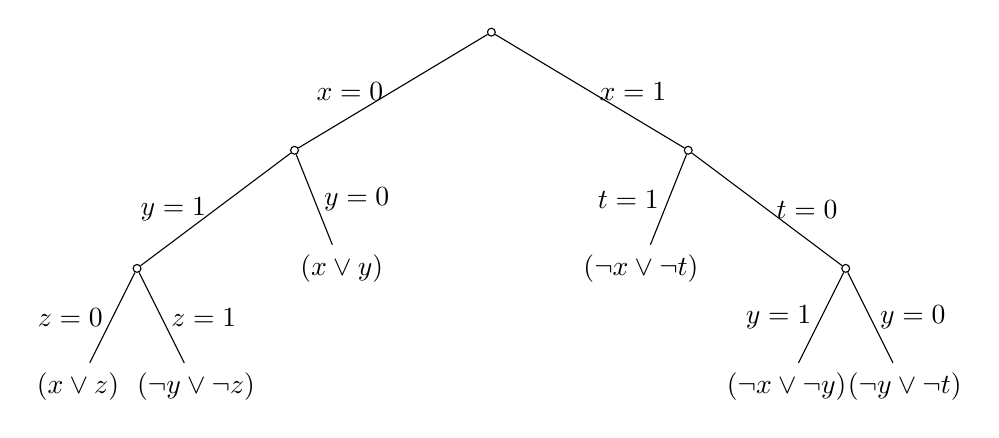
\begin{tikzpicture}[label distance=8mm]
	\node [end] {}
        child {
        	node[end] {}
           	child {
               	node[end] {}
               	child {
                	node {\alert{$(x \lor z)$}}
	                edge from parent
		            node[left] {$z = 0$}
	            }
			    child {
	                node {\alert{$(\neg y \lor \neg z)$}}
	                edge from parent
		            node[right] {$z = 1$}
	            }
                edge from parent
	            node[left] {$y = 1$}
            }
            child[sibling distance = 1.2cm] {
               	node {\alert{$(x \lor y)$}}
                edge from parent
	            node[right] {$y = 0$}
            }
           	edge from parent
            node[left] {$x = 0$}
        }
        child {
        	node[end] {}
            child[sibling distance = 1.2cm] {
            	node {\alert{$(\neg x \lor \neg t)$}}
                edge from parent
                node[left] {$t = 1$}
            }
            child {
            	node[end] {}
                child {
            		node {\alert{$(\neg x \lor \neg y)$}}
	                edge from parent
    	            node[left] {$y = 1$}
        	    }
                child {
            		node {\alert{$(\neg y \lor \neg t)$}}
                	edge from parent
	                node[right] {$y = 0$}
    	        }
                edge from parent
                node[right] {$t = 0$}
            }
           	edge from parent
            node[right] {$x = 1$}
        };
\end{tikzpicture}

%%% Local Variables: 
%%% mode: latex
%%% TeX-master: t
%%% End: 
}
	\only<2>{\tikzstyle{end} = [circle, minimum size = 0.1cm, draw, inner sep = 0.1pt]
\tikzstyle{leaf} = [circle, minimum size = 0.6cm, draw, inner sep = 0.1pt, blue]
            
\tikzstyle{level 1}=[level distance = 1.5cm, sibling distance = 5cm]
\tikzstyle{level 2}=[sibling distance = 4cm]
\tikzstyle{level 3}=[sibling distance = 1.5cm]
    
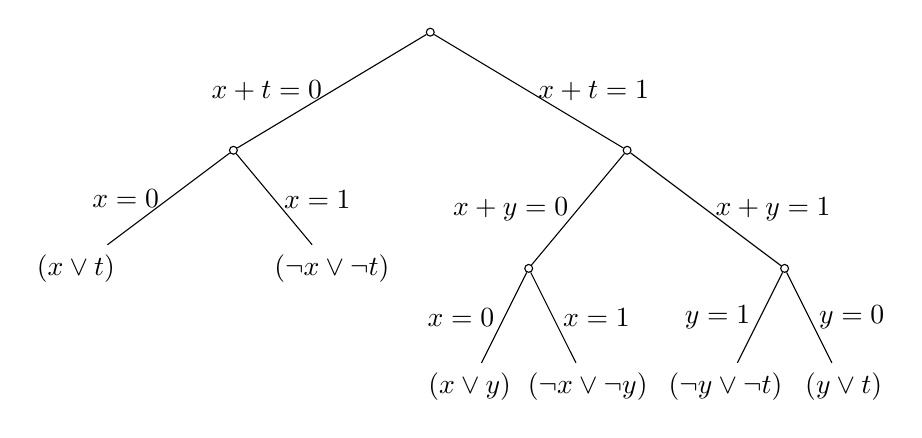
\begin{tikzpicture}[label distance=8mm]
	\node [end] {}
        child {
        	node[end] {}
           	child {
               	node {\alert{$(x \lor t)$}}
                edge from parent
	            node[left] {$x = 0$}
            }
            child[sibling distance = 2.5cm] {
               	node {\alert{$(\neg x \lor \neg t)$}}
                edge from parent
	            node[right] {$x = 1$}
            }
           	edge from parent
            node[left] {$x + t = 0$}
        }
        child {
        	node[end] {}
            child[sibling distance = 2.5cm] {
                node[end] {}
                child {
            		node {\alert{$(x \lor y)$}}
	                edge from parent
    	            node[left] {$x = 0$}
        	    }
                child {
            		node {\alert{$(\neg x  \lor \neg y)$}}
                	edge from parent
	                node[right] {$x = 1$}
    	        }
                edge from parent
                node[left] {$x + y = 0$}
            }
            child {
            	node[end] {}
                child {
            		node {\alert{$(\neg y \lor \neg t)$}}
	                edge from parent
    	            node[left] {$y = 1$}
        	    }
                child {
            		node {\alert{$(y \lor t)$}}
                	edge from parent
	                node[right] {$y = 0$}
    	        }
                edge from parent
                node[right] {$x + y = 1$}
            }
           	edge from parent
            node[right] {$x + t = 1$}
        };
\end{tikzpicture}

%%% Local Variables: 
%%% mode: latex
%%% TeX-master: t
%%% End: 
}
\end{frame}


\begin{frame}
    \frametitle{Алгоритм Сето и Тамаки}

	\begin{itemize}
		\item{} [Seto, Tamaki, 2011] Алгоритм для Formula-SAT над полным бинарным базисом. Для формул размера $cn$ алгоритм
		    работает $2^{(1 - \mu_c)n}$ шагов, где $\mu_c$~--- константа.
        \pause
		\item Алгоритм использует расщепление по линейным комбинациям.
	\end{itemize}    
\end{frame}


\begin{frame}
    \frametitle{Верхние оценки}

    \begin{itemize}
		\item Линейные системы над $\mathbb{F}_2$:
			\begin{itemize}
				\item трудны для резолюций;
				\item просты для LST.
			\end{itemize}
        \pause
		\item Perfect matching principle для графов с нечетным числом вершин:
		    \begin{itemize}
        		\item трудны для резолюций [Разборов, 2003];
				\item просты для LST.
			\end{itemize}
        \pause
		\item Игры с фишками.
			\begin{itemize}
				\item Пусть $\phi$ формула в КНФ обозначим за $\phi^{\oplus}$ КНФ формулу, полученную из $\phi$ путем подстановки
		            $x_1 \oplus x_2$ для каждой переменной $x$. 
				\item{} [Urquhart, 2011] Размер древесного вывода в резолюциях $\phi^{\oplus}$ не менее $2^{d(\phi)}$, где
		            $d(\phi)$ минимальная глубина резолюционного вывода для  $\phi$.
				\item{} [Urquhart, 2011] Для игры с фишками $Peb(G_n)$ выполнено: $d(Peb(G_n)) = \Omega(n / \log(n))$ и $Peb(G_n)$
		            имеет $O(n)$ древесный резолюционный вывод.
				\item Древесный резолюционный вывод для $Peb^\oplus(G_n)$ не менее $2^{n / \log n}$, но $Peb^\oplus(G_n)$ имеет
		            LST размера $O(n)$. 
			\end{itemize}
	\end{itemize}
\end{frame}



\begin{frame}
    \frametitle{Линейные системы}

    \begin{columns}
		\begin{column}{1cm}
			Невыполнимая система:

			$\left\{ \begin{aligned}
				f_1 = \alpha_1 \\
				f_2 = \alpha_2 \\
				\dots\\
				f_m = \alpha_m
			\end{aligned}\right.$
		\end{column}


	\begin{column}{9cm}
			\tikzstyle{end} = [thin, circle, minimum size = 0.1cm, draw, inner sep = 0.1pt]
\tikzstyle{leaf} = [thin, circle, minimum size = 0.6cm, draw, inner sep = 0.1pt, blue]
            
\tikzstyle{level 1}=[level distance = 1.5cm, sibling distance = 1.5cm]
\tikzstyle{level 2}=[level distance = 1.5cm, sibling distance = 4cm]
\tikzstyle{level 3}=[level distance = 2cm, sibling distance = 1.5cm]
\tikzstyle{level 4}=[level distance = 2cm, sibling distance = 1.3cm]

\tikzstyle{edge from parent} = [thin, draw]

    
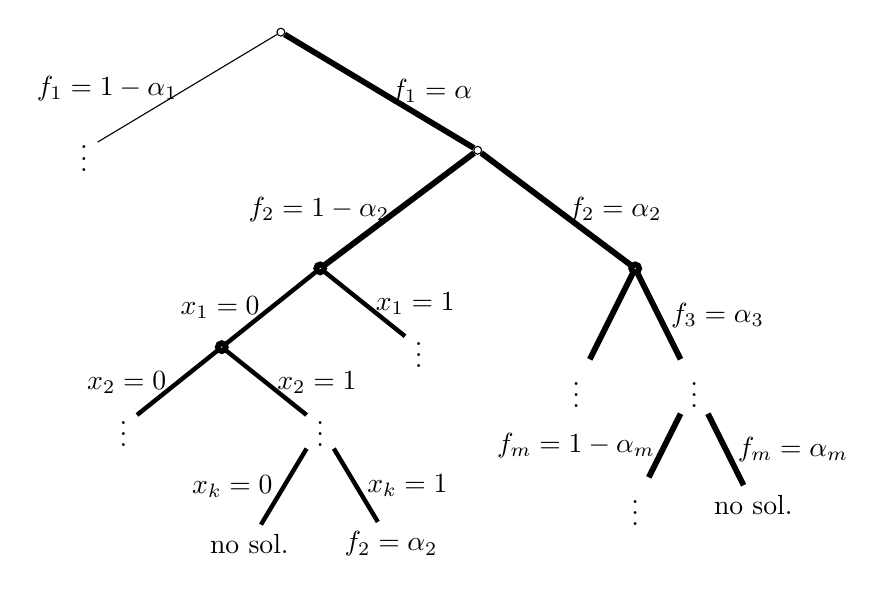
\begin{tikzpicture}[label distance = 8mm]
	\node [end] {}
	    child {
        	node {$\vdots$}
           	edge from parent
            node[left] {$f_1 = 1 - \alpha_1$}
        }
        child {
        	node[end] {}
            child {
		        node[end] {}
                child[level distance = 1.cm, sibling distance = 2.5cm] {
        			node[end] {}
                    child[level distance = 1cm] {
                    	node {$\vdots$}
                    	edge from parent[ultra thick]
	        		    node[left] {$x_2 = 0$}
                    }
                    child[level distance = 1cm] {
                    	node {$\vdots$}
                        child[level distance = 1.5cm, sibling distance = 1.8cm] {
                        	node {\alert{no sol.}}
                            edge from parent[ultra thick]
		        		    node[left] {$x_k = 0$}
                        }
                        child[level distance = 1.5cm, sibling distance = 1.8cm] {
                        	node {\alert{$f_2 = \alpha_2$}}
                            edge from parent[ultra thick]
		        		    node[right] {$x_k = 1$}
                        }
                    	edge from parent[ultra thick]
	        		    node[right] {$x_2 = 1$}
                    }
		           	edge from parent[ultra thick]
        		    node[left] {$x_1 = 0$}
		        }
                child[level distance = 1.cm, sibling distance = 2.5cm] {
                  	node {$\vdots$}
                    edge from parent[ultra thick]
                    node[right] {$x_1 = 1$}
                }
	            edge from parent
		        node[left] {$f_2 = 1 - \alpha_2$}
			}
		    child {
		        node[end] {}
                child {
        			node {$\vdots$}
		           	edge from parent
        		    node[left] {}
		        }
                child {
                  	node {$\vdots$}
                    child{
  		                node {$\vdots$}
			           	edge from parent
        			    node[left] {$f_m = 1 - \alpha_m$}
                    }
                    child{
  		                node {\alert{no sol.}}
			           	edge from parent[line width = 2.1pt]
        			    node[right] {$f_m = \alpha_m$}
                    }
                    edge from parent[line width = 2.1pt]
                    node[right] {$f_3 = \alpha_3$}
                }
	            edge from parent[line width = 2.1pt]
		        node[right] {$f_2 = \alpha_2$}
            }
           	edge from parent[line width = 2.1pt]
            node[right] {$f_1 = \alpha$}
        };
\end{tikzpicture}

%%% Local Variables: 
%%% mode: latex
%%% TeX-master: t
%%% End: 

		\end{column}
	\end{columns}

	$f_2 = x_1 + \dots + x_k$
\end{frame}




\begin{frame}
    \frametitle{$\ResL$}

    \begin{itemize}
		\item Литерал: $L = x_{1} + x_{2} + \dots + x_{k} = \alpha$,
    		$\lnot L = x_{1} + x_{2} + \dots + x_{k} = \alpha + 1$
		\item Линейный клоз: $\bigvee_i x_{i, 1} + x_{i, 2} + \dots + x_{i, k_i} =
		    \alpha_i$ или $\lnot \bigwedge x_{i, 1} + x_{i, 2} + \dots + x_{i, k_i} =
            1 + \alpha_i$.
        \pause
		\item $\ResL$:
			\begin{itemize}
				\item Правило резолюции: $\frac{(f = 0) \lor D, (f = 1) \lor D'}
            		{D \lor D'}$ 
				\item Правило ослабления: $\frac{C}{C'}$ если $C$ семантически влечет $C'$
			\end{itemize}
        \pause
		\item \mycolor{blue}{Древовидная} $\ResL$ эквивалента LST.
	\end{itemize}
	\scalebox{0.8}{\tikzstyle{end} = [circle, minimum size = 0.1cm, draw, inner sep = 0.1pt]
\tikzstyle{leaf} = [circle, minimum size = 0.6cm, draw, inner sep = 0.1pt, blue]


\onslide<1->{
	\tikzstyle{level 1}=[level distance = 1.5cm, sibling distance = 6cm, opacity = 0]
	\tikzstyle{level 2}=[sibling distance = 3cm, opacity = 0]
}
\only<3->{
	\tikzstyle{level 1}=[level distance = 1.5cm, sibling distance = 6cm, opacity = 1]
	\tikzstyle{level 2}=[sibling distance = 3cm, opacity = 1]
}






    
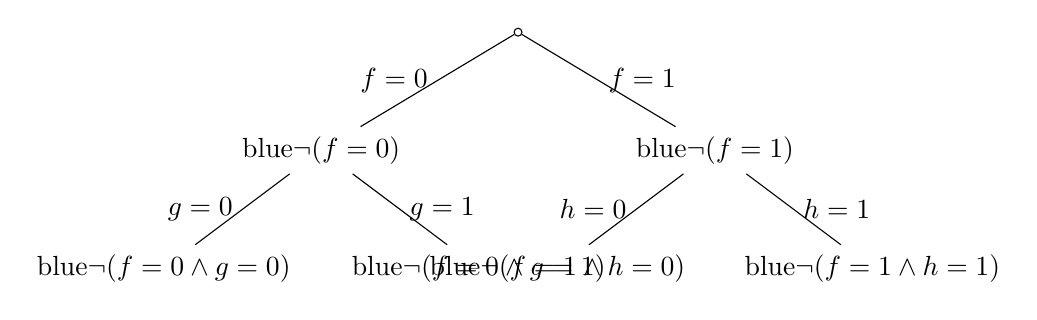
\begin{tikzpicture}[label distance = 8mm, all/.style = {opacity = 0}]
	\node [end] {}
        child {
            node {\mycolor{blue}{$\neg (f = 0)$}}
           	child {
                node {\mycolor{blue}{$\neg (f = 0 \land g = 0)$}}
                edge from parent
	            node[left] {$g = 0$}
            }
            child {
               	node {\mycolor{blue}{$\neg (f = 0 \land g = 1)$}}
                edge from parent
	            node[right] {$g = 1$}
            }
           	edge from parent
            node[left] {$f = 0$}
        }
        child {
            node {\mycolor{blue}{$\neg (f = 1)$}}
           	child {
                node {\mycolor{blue}{$\neg (f = 1 \land h = 0)$}}
                edge from parent
	            node[left] {$h = 0$}
            }
            child {
               	node {\mycolor{blue}{$\neg (f = 1 \land h = 1)$}}
                edge from parent
	            node[right] {$h = 1$}
            }
           	edge from parent
            node[right] {$f = 1$}
        };
\end{tikzpicture}

%%% Local Variables: 
%%% mode: latex
%%% TeX-master: t
%%% End: 
}
\end{frame}



\begin{frame}
    \frametitle{$\ResL$ vs $\SemL$}

    \begin{itemize}
		\item $\SemL$:
			\begin{itemize}
				\item Семантическое правило: $\frac{C_1, C_2}{C'}$ если $C_1 \land C_2$
		            семантически влечет $C'$
				\item Правило ослабления: $\frac{C}{C'}$ если $C$ семантически влечет $C'$
			\end{itemize}
	\end{itemize}

	\pause
    \begin{theorem}
        $\ResL$ p-моделирует $\SemL$.
    \end{theorem}
\end{frame}

\begin{frame}
    \frametitle{Нижняя оценка на 2-сложенные Цейтинские формулы}

    \begin{itemize}
		\item Невыполнимая формула $\phi$ $\Rightarrow$ задача $Search_\phi$: найти невыполненный клоз по подстановке
		    значений переменным.
        \pause 
		\item LST $T$ $\Rightarrow$ вероятностный коммуникационный протокол для $Search_\phi$ глубины $O(\log |T|
		    \log\log |T|)$ (некоторые значения знает Алиса, некоторые Боб).
        \pause
		\item Применяем нижнюю оценку на вероятностную коммуникационную сложность $Search_{TS^2_{G,c}}$ для 2-сложенных
		    Цейтинских формул $TS^2_{G,c}$ ([Kalyanasundaram, Schintger 1992] и [Beame, Pitassi, Segerlind, 2007]).
	\end{itemize}
	\pause
    \begin{theorem}
        Существует явная конструкция графа такого $G(V, E)$ на $n$ вершинах с константной степенью и функций $c: V \to
        \mathbb{F}_2$, что размер LST для $TS^2_{(G,c)}$ равен $\Omega\left(2^{n^{1 / 3} / \log^3(n)} \right)$.
    \end{theorem}
\end{frame}


\begin{frame}
    \frametitle{Открытые вопросы}

    \begin{itemize}
        \item Доказательство нижней оценки для явной конструкции функции Голдрейха и случайного предиката.
        \item Доказательство компромисса между корректностью и временем работы $\DPLL$ алгоритмов с ошибкой для случая
    		вероятностной процедуры $A$.
		\item Доказательство нижних оценок на $\ResL$ (не древесных).
		\item Соотношение между $\ResL$ и другими известными системами доказательств.
		\item Доказательство нижних оценок на LST для \mycolor{blue}{выполнимых} формул.
	\end{itemize}
\end{frame}


%%% Local Variables: 
%%% mode: latex
%%% TeX-master: t
%%% End: 
